\documentclass[openany,12pt,a4paper]{report}
\usepackage{subfiles}
\usepackage[]{graphicx}
\usepackage{float}
\usepackage{multirow}
\graphicspath{{./img/}{./../img/}}
\usepackage{../StileDoc}
\title{Product Baseline - Allegato tecnico}
\author{}

\loadglsentries{../Glossario/Definizioni}
%Ultima versione documento

\newcommand{\versione}{0.0.0}


\begin{document}
	\makeatletter
	\begin{titlepage}
		\setlength{\headsep}{0pt}  
		\begin{center}
			
\includegraphics[width=0.5\linewidth]{img/logo.png}\\[1em]
			{\huge \bfseries  \@title }\\[10ex]
			\textbf{\Large Informazioni Documento} \\[2em]
			\bgroup
			\def\arraystretch{1.5}
			\begin{tabular}{l|l}
				\textbf{Data approvazione} & 10 Marzo 2018 \\
				\textbf{Responsabile} & Marco Focchiatti\\
				\textbf{Redattori} &  Manfredi Smaniotto, Marco Focchiatti,\\
				& Cristiano Tessarolo, Giulio Rossetti, \\
				& Kevin Silvestri \\
				\textbf{Verificatori} & Manfredi Smaniotto, Marco Focchiatti \\
				\textbf{Distribuzione} & Prof. Tullio Vardanega \\
				& Prof. Riccardo Cardin \\
				& Gruppo Graphite \\
				\textbf{Uso} & Esterno \\
				\textbf{Recapito} & graphite.swe@gmail.com \\
			\end{tabular}
			\egroup
		\end{center}
	\end{titlepage}
	\makeatother
	
	\thispagestyle{empty}
	\newpage
	
	%REGISTRO DELLE MODIFICHE
	
	\chapter*{Registro delle modifiche}
	\setlength\LTleft{-22mm}
	\begin{longtable}{|p{20mm}|p{20mm}|p{40mm}|p{30mm}|p{50mm}|}
		\hline
		\textbf{Versione} & \textbf{Data} & \textbf{Autore} & \textbf{Ruolo} & \textbf{Descrizione} \\
		
		\hline 2.0.0 & 10-03-2018 & Marco Focchiatti & Responsabile & Approvazione \\
		\hline 1.2.0 & 09-03-2018 & Giulio Rossetti & Verificatore & Verifica \\
		\hline 1.1.1 & 08-03-2018 & Kevin Silvestri & Verificatore & Stesura appendice §C.3 e §D  \\
		\hline 1.1.0 & 25-02-2018 & Marco Focchiatti & Verificatore & Verifica \\
		\hline 1.0.6 & 23-02-2018 & Manfredi Smaniotto & Verificatore & Stesura appendice §B \\
		\hline 1.0.5 & 22-02-2018 & Manfredi Smaniotto & Verificatore & Spostamento appendice §B in appendice §C \\
		\hline 1.0.4 & 16-02-2018 & Giulio Rossetti & Verificatore & Rivisto e modificato §3 \\
		\hline 1.0.3 & 13-02-2018 & Cristiano Tessarolo & Verificatore & Rivisti obiettivi di qualità (§2.2) e aggiunta politica della qualità (§2.4) \\
		\hline 1.0.2 & 11-02-2018 & Kevin Silvestri & Verificatore & Spostate definizioni metriche (§3) in NP\\
		\hline 1.0.1 & 09-02-2018 & Marco Focchiatti & Verificatore & Rivista struttura generale e ampliata §2 \\
		\hline 1.0.0 & 12-01-2018 & Samuele Modena & Responsabile & Approvazione \\
		\hline 0.2.0 & 11-01-2018 & Giulio Rossetti & Verificatore & Verifica \\
		\hline 0.1.2 & 10-01-2018 & Samuele Modena & Verificatore & Stesura appendice §B \\
		\hline 0.1.1 & 20-12-2017 & Matteo Rizzo & Verificatore & Aggiornata §3 \\
		\hline 0.1.0 & 19-12-2017 & Manfredi Smaniotto & Verificatore & Verifica \\		
		\hline 0.0.6 & 18-12-2017 & Kevin Silvestri & Verificatore & Stesura appendice §A \\
		\hline 0.0.5 & 17-12-2017 & Kevin Silvestri & Verificatore & Stesura §4 \\	
		\hline 0.0.4 & 15-12-2017 & Matteo Rizzo & Verificatore & Stesura §3 \\
		\hline 0.0.3 & 14-12-2017 & Samuele Modena & Verificatore & Stesura §2 \\
		\hline 0.0.2 & 13-12-2017 & Matteo Rizzo & Verificatore & Stesura §1 \\
		\hline 0.0.1 & 13-12-2017 & Matteo Rizzo & Verificatore & Creazione del template \\
		\hline
		
	\end{longtable}
	
	\tableofcontents
	
	\chapter{Introduzione}
	
	\section{Scopo del documento}
	
	Il documento ha la finalità di illustrare la \textit{Product Baseline} (PB in breve) per l’applicazione
	\textit{"DeSpeect: un'interfaccia grafica per Speect"}, con particolare attenzione per lo stato attuale del prodotto, la sua architettura e la copertura di use case e requisiti funzionali obbligatori.
	
	\section{Scopo del prodotto}
	
	Lo scopo del progetto è la realizzazione di un’interfaccia grafica per \glossario{Speect}{Speect} [Meraka Institute(2008-2013)], una libreria per la creazione di sistemi di sintesi vocale, che agevoli l’ispezione del suo stato interno durante il funzionamento e la scrittura di test per le sue funzionalità.


	\section{Riferimenti}
	
	\subsection*{Riferimenti normativi}
	
	\begin{itemize}
		\item \textbf{Norme di Progetto v3.0.0}: documento \textit{Norme di progetto v3.0.0};
		\subitem §2.2.5 "Progettazione";
		\subitem §4.7.3 "Strumenti relativi allo sviluppo".
	\end{itemize}
	
	\subsection*{Riferimenti informativi}
	
	\begin{itemize}
		\item \textbf{Analisi dei Requisiti v3.0.0}: documento \textit{Analisi dei Requisiti v3.0.0};
		\subitem Definisce nel dettaglio use case e requisiti.
		
		\item \textbf{Documentazione Speect:} \\
		\url{http://speect.sourceforge.net/contents.html};
		\subitem Documentazione ufficiale della libreria di \textit{Text-To-Speech} di riferimento per il progetto.
		
		\item \textbf{Documentazione Qt:} \\
		\url{http://doc.qt.io/};
		\subitem Documentazione ufficiale del framework utilizzato per lo sviluppo dell'interfaccia grafica.
		
		\item \textbf{Documentazione CMAKE:} \\
		\url{https://cmake.org/documentation/}.
		\subitem Documentazione ufficiale del framework utilizzato per la build del prodotto. 
	\end{itemize}

	\chapter{Requisiti di sistema}
	
	L'installazione ed esecuzione del software richiede i seguenti prerequisiti:
	
	\begin{itemize}
		\item Sistema operativo Unix / Unix-like (il software è stato testato solo per piattaforma Ubuntu 16.04 LTS)
		\subitem \url{https://www.ubuntu.com/download/desktop}
		\item CMake (versione minima 2.8)
		\subitem \url{https://cmake.org/download/}
		\item Compilatore ANSI C/ISO C90 GCC (versione minima 5.0)
		\subitem \url{https://gcc.gnu.org/install/binaries.html}
		\item Qt 5.9.0
		\subitem \url{https://www.qt.io/download}
	\end{itemize}

	\chapter{Installazione ed esecuzione}
	
	Il codice relativo alla Product Baseline è reperibile da un apposito repository GitHub al seguente link:
	\begin{center}
		\url{https://github.com/graphiteSWE/Despeect-ProductBaseline}
	\end{center} 

	\noindent Per installare ed eseguire il software è necessario attenersi alla seguente procedura:
	\begin{enumerate}
		\item Clonare o scaricare la repository sulla propria macchina;
		\item Entrare nella cartella scaricata ed eseguire lo script \verb|build.sh|;
		\item Eseguire da terminale il comando \verb|cd DeSpeect/build/|;
		\item Avviare l'eseguibile con il comando \verb|./main|.
	\end{enumerate}
	Tale procedura installerà la libreria Speect e genererà una build del software nella directory \verb|DeSpeect/build|, nonché avvierà automaticamente un'esecuzione dello stesso. Ulteriori informazioni sono reperibili nel file \verb|README.md| del repository.

	\chapter{Rapporto con il PoC}
	Precedentemente alla Product Baseline, è stato realizzato un \textit{Proof of Concept} (PoC in breve) a dimostrazione della fattibilità del prodotto DeSpeect. Tale PoC è tuttora reperibile al seguente link:
	\begin{center}
		\url{https://github.com/graphiteSWE/TB-PoC}
	\end{center}

	\noindent Segue una tabella che evidenzia le differenze tra le caratteristiche del PoC, contestualizzato nel suo scopo, e quelle della PB. \\
	
	\begin{longtable}{|p{80mm}|p{80mm}|}
		\caption {Tabella di confronto tra PoC e PB} \label{tab:Tabella di confronto tra PoC e PB} \\
		\hline
		\textbf{Proof of Concept} & \textbf{Product Baseline} \\
		
		\hline Architettura abbozzata e sommaria, priva di design pattern 
		&
		Architettura basata su MVVM e facente uso di vari design pattern \\ 
		
		\hline Implementazione di un'interfaccia grafica provvisoria e carente di elementi fondamentali per il soddisfacimento di molti requisiti obbligatori 
		&
		Interfaccia grafica quasi completa predisposta all'implementazione della totalità dei requisiti obbligatori \\ 
		
		\hline Implementazione di poche funzionalità dimostrative (per esempio la stampa parziale del grafo)
		&
		Implementazione della maggior parte delle funzionalità richieste dai requisiti funzionali obbligatori \\ 
		
		\hline Modalità di installazione e configurazione macchinose
		&
		Modalità di installazione e configurazione semplificate \\ 
		\hline
	\end{longtable}

	\chapter{Architettura}
	
	\section{Model-View-ViewModel}
	
	\section{Model}
		
	\subsection{Design pattern}
	
	\subsubsection{Command}
	
	\subsubsection{Builder}
	
	\subsubsection{Adapter}
	
	\section{View}
	
	\section{ViewModel}
	
	\subsubsection{Observer}
	
	\subsection{Design pattern}

	\chapter{Use case coperti}
	
	\section{Tabella della copertura degli use case}
	
	\section{Grafico della copertura degli use case}
	
	\chapter{Requisiti soddisfatti}
	
	\section{Tabella del soddisfacimento dei requisiti}
	
	\section{Grafico del soddisfacimento dei requisiti}
	
	\appendix
	
	\chapter{Model-View-ViewModel}
	
	\section{Struttura del pattern}
	
	Il design pattern architetturale \textit{Model-View-ViewModel} (MVVM in breve) facilita la separazione dell'interfaccia grafica, che si tratti di linguaggio di markup o codice GUI, dallo sviluppo della logica di business o della logica di back-end, ovvero dal modello dei dati. Il \textit{view model} di MVVM è un convertitore di valori, nel senso che il view model è responsabile dell'esposizione (conversione) degli oggetti dati dal modello così da renderli facilmente gestibili e presentabili. In quest'ottica, la view è più un modello che una vista e gestisce la maggior parte se non tutta la logica di visualizzazione della vista. Il pattern è riassunto dal seguente schema ed i suoi componenti principali sono di seguito approfonditi.\\
	
	\begin{figure}[H]
		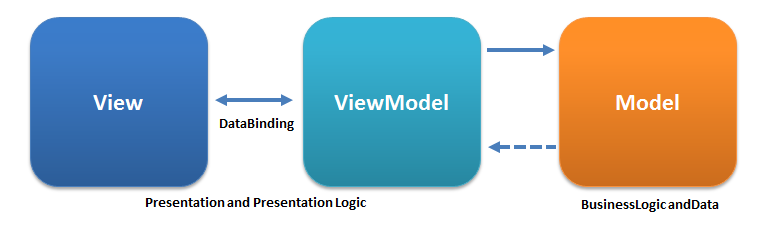
\includegraphics[scale=0.7]{MVVMPattern}
		\centering
		\caption{Diagramma generale dell'architettura MVVM}
	\end{figure}
	
	\noindent I tre componenti principali dell'architettura sono i seguenti:
	\begin{itemize}
		\item \textbf{Model}: il \textit{Model} (o modello) è un'implementazione del modello di dominio dell'applicazione ed include un modello dei dati affiancato alla logica di business e di validazione;
		\item \textbf{View}: la \textit{View} (o vista) è responsabile della definizione della struttura, del layout e dell'aspetto di ciò che l'utente visualizza su schermo. Idealmente, la vista è definita puramente con linguaggio di markup o generico codice GUI che non contiene la logica di business;
		\item \textbf{ViewModel}: la \textit{ViewModel} (o modello di presentazione) funge da intermediario tra la vista e il modello ed è responsabile della gestione della logica di visualizzazione. In genere, il ViewModel interagisce con il modello richiamandone i metodi delle classi: esso fornisce quindi dati dal modello in una forma facilmente utilizzabile dalla View. Il ViewModel recupera i dati dal modello, rendendoli disponibili alla View, e può riformattarli in un modo che renda più semplice la gestione della vista. Esso fornisce anche l'implementazione dei comandi che un utente dell'applicazione avvia nella vista (ad esempio, quando un utente clicca un pulsante nell'interfaccia grafica, tale azione può attivare un comando nel ViewModel) e può essere responsabile della definizione delle modifiche dello stato logico che influiscono su alcuni aspetti della visualizzazione nella vista, ad esempio l'indicazione che alcune operazioni sono in sospeso.
	\end{itemize}

	\section{Vantaggi offerti dal pattern}
	Il MVVM offre i seguenti vantaggi:
	
	\begin{itemize}
		\item Durante il processo di sviluppo, i programmatori e i designer possono lavorare in modo indipendente e simultaneamente sui loro componenti. Quest'ultimi possono concentrarsi sulla vista e, utilizzando appositi strumenti, generare facilmente dati di esempio con cui lavorare, mentre i programmatori possono lavorare sul modello di presentazione e sui componenti del modello;
		\item Gli sviluppatori possono creare test unitari per il ViewModel e per il Model senza utilizzare la View;
		\item È facile riprogettare l'interfaccia grafica dell'applicazione senza toccare il resto del codice, una nuova versione della vista dovrebbe poter funzionare con il modello di presentazione esistente;
		\item Se esiste un'implementazione del modello che incapsula la logica di business, potrebbe essere difficile o rischioso cambiarla. In questo scenario, il ViewModel funge da adattatore per le classi del Model e consente di evitare modifiche importanti al codice dello stesso.	
	\end{itemize}
	
	\chapter{Design Pattern}
	
	Vengono di seguito illustrati sinteticamente i design pattern implementati dal prodotto DeSpeect.
	
	\section{Command}
	
	Il Command pattern è un design pattern che permette di isolare la porzione di codice che effettua un'azione (eventualmente molto complessa) dal codice che ne richiede l'esecuzione; l'azione è incapsulata nell'oggetto Command. L'obiettivo è rendere variabile l'azione del client senza però conoscere i dettagli dell'operazione stessa. Altro aspetto importante è che il destinatario della richiesta può non essere deciso staticamente all'atto dell'istanziazione del comando ma ricavato a tempo di esecuzione. Segue il diagramma UML rappresentativo del pattern. \\
	
	\begin{figure}[H]
		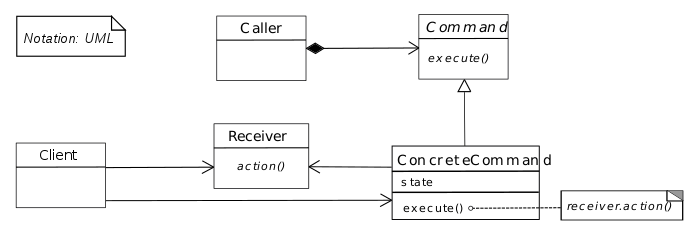
\includegraphics[scale=0.6]{CommandPattern}
		\centering
		\caption{Diagramma UML del design pattern Command}
	\end{figure}
	
	\section{Builder}
	
	\section{Adapter}
	
	\section{Observer}
	
\end{document}